\documentclass[twoside,twocolumn]{article}

\usepackage{blindtext} % Package to generate dummy text throughout this template 
\usepackage{graphicx}
\usepackage[sc]{mathpazo} % Use the Palatino font
\usepackage[T1]{fontenc} % Use 8-bit encoding that has 256 glyphs
\linespread{1.05} % Line spacing - Palatino needs more space between lines
\usepackage{microtype} % Slightly tweak font spacing for aesthetics

\usepackage[english]{babel} % Language hyphenation and typographical rules

\usepackage[hmarginratio=1:1,top=32mm,columnsep=20pt]{geometry} % Document margins
\usepackage[hang, small,labelfont=bf,up,textfont=it,up]{caption} % Custom captions under/above floats in tables or figures
\usepackage{booktabs} % Horizontal rules in tables

\usepackage{lettrine} % The lettrine is the first enlarged letter at the beginning of the text

\usepackage{enumitem} % Customized lists
\setlist[itemize]{noitemsep} % Make itemize lists more compact

\usepackage{abstract} % Allows abstract customization
\renewcommand{\abstractnamefont}{\normalfont\bfseries} % Set the "Abstract" text to bold
\renewcommand{\abstracttextfont}{\normalfont\small\itshape} % Set the abstract itself to small italic text

\usepackage{titlesec} % Allows customization of titles
\renewcommand\thesection{\Roman{section}} % Roman numerals for the sections
\renewcommand\thesubsection{\roman{subsection}} % roman numerals for subsections
\titleformat{\section}[block]{\large\scshape\centering}{\thesection.}{1em}{} % Change the look of the section titles
\titleformat{\subsection}[block]{\large}{\thesubsection.}{1em}{} % Change the look of the section titles

\usepackage{fancyhdr} % Headers and footers
\pagestyle{fancy} % All pages have headers and footers
\fancyhead{} % Blank out the default header
\fancyfoot{} % Blank out the default footer
\fancyhead[L]{Comparativa de Gestiores de BD NoSQL } % Custom header text
\fancyhead[R]{November 2020 } % Custom header text
\fancyfoot[RO,LE]{\thepage} % Custom footer text

\usepackage{titling} % Customizing the title section

\usepackage{hyperref} % For hyperlinks in the PDF

%----------------------------------------------------------------------------------------
%	TITLE SECTION
%----------------------------------------------------------------------------------------

\setlength{\droptitle}{-4\baselineskip} % Move the title up

\pretitle{\begin{center}\Huge\bfseries} % Article title formatting
\posttitle{\end{center}} % Article title closing formatting
\title{COMPARATIVA DE GESTORES DE BASE DE DATOS NO RELACIONALES} % Article title
\author{Arias, Cancino, Crispin, Gutierrez, Zuñiga} 
\date{\today} % Leave empty to omit a date
\renewcommand{\maketitlehookd}{%
\begin{abstract}
	\begin{center}
		\textbf{Resumen}
	\end{center}
	Las bases de datos NoSQL, forman una agrupación dentro de las bases de datos, diferenciándose de las demás al no seguir al modelo de bases de datos relacionales y sus propiedades. Las bases de datos NoSQL hacen referencia a variedad de bases de datos que tienen el propósito de solventar algunas limitaciones que el modelo relacional presenta, se caracterizan por no tener esquemas, no usan SQL como parte fundamental en el lenguaje de consultas, no aseguran cumplir con la propiedad ACID , los datos almacenados en una BD no requieren necesariamente cumplir con estructuras fijas como tablas, por lo regular no sostienen operaciones de tipo JOIN y tienden a tener un escalamiento horizontal, ocupan un extenso recurso de la memoria principal del ordenador, solventan las dificultades en el elevado volumen de información y las innumerables cantidades de consultas y transacciones que se realizan de forma diaria.
\\
	\begin{center}
		
		\textbf{Abstract}
	\end{center}
	NoSQL databases form a grouping within databases, differentiating themselves from the others by not following the relational database model and its properties. NoSQL databases refer to a variety of databases that have the purpose of solving some limitations that the relational model presents, they are characterized by not having schemas, they do not use SQL as a fundamental part in the query language, they do not claim to comply with the ACID property, the data stored in a DB does not necessarily have to comply with fixed structures such as tables, they usually do not support JOIN type operations and tend to have horizontal scaling, they occupy an extensive resource of the computer's main memory, they solve the difficulties in the high volume of information and the innumerable amounts of inquiries and transactions that are carried out on a daily basis.
	\\
\end{abstract}
}
%----------------------------------------------------------------------------------------

\begin{document}
% Print the title
\maketitle
\vspace*{5 in}
\section{Introducción}
El mundo de las bases de datos ha cambiado vertiginosamente sus rumbos, desde el mundo de las bases de datos relacionales hacia el mundo NoSQL. 
En éstos capítulos se exponen el origen y fundamentos de las bases de datos tipo NoSQL.
El articulo completo pretende entregar los elementos claves de éstos motores, su forma de trabajo, como se instalan y que consideraciones se deben tener presente para el uso de éstas. Cabe señalar que las bases de datos de tipo NoSQL surgen de la necesidad de usuarios y empresas de realizar transacciones con un alto rendimiento y performance bajo una filosofía distinta a las bases de datos relacionales.
\\
\section{Desarrollo}
\textbf{¿Qué son las Bases de Datos NoSql?}
Corresponden a bases de datos diseñadas y pensadas para aplicaciones que hagan un uso intensivo de la información, es decir operen y manipulen con un gran volumen de datos.
La filosofía de estas bases de datos es que se alojan en la RAM no en un disco duro.
\\
Existen un sin número de bases de datos del tipo NoSQL como, por ejemplo: \\
\begin{center}
    \textbf{MongoDB (usa JSON), Redis, Cassandra}\\
\end{center}
Cada una de éstas tiene una forma de operar distinta y un modo de consola para ejecutar comandos que son diferentes, pero que tienen como objetivo realizar transacciones rápidas y efectivas.\\

\textbf{Características:}\\
El término NoSQL fue desarrollado en 1990 por C. Strozzi, pero su implementación comenzó a ejecutarse a partir del año 2009. El término NoSQL se puede interpretar como Not Only SQL (No Sólo SQL, en español).
\\
La gran cantidad de información manejada en comunidades, redes sociales, buscadores, y muchos otros proyectos en el ámbito de la Web 2.0 fue altísima, lo que ha hecho que surjan nuevas arquitecturas de almacenamiento de información, que deben ser de alto rendimiento, escalables y distribuidas.
\\

\textbf{Orígenes:}\\
\begin{itemize}
    \item Estas bases de datos permiten una mayor flexibilidad y facilidad a la hora de introducir los datos y funcionan con mayor rapidez a la hora de solicitar datos. 
    \item La mayoría de las bases de datos NoSql son montadas normalmente en clusters, es decir, se alojan en la RAM no en el disco duro, por lo que llevan a cabo las operaciones en nanosegundos en lugar de milisegundos. Razón por la cual son tan rápidas.
    \item Además son tolerante a fallos, presentan escalabilidad horizontal.
    \item El auge actual de este tipo de base de datos viene determinado por el uso de gran cantidad de datos en empresas como Amazon, Google, Twitter y Facebook.
    \item Muchas bases de datos del tipo NoSQL son de uso libre y pueden bajarse desde la web, o del sitio oficial de sus partners o proveedores.
    \item Las bases de datos NoSQL son listas de datos almacenados en una sola tabla sin definir relaciones entre los registros.
    \item A diferencia de las bases de datos relacionales reparten los datos en varias tablas más pequeñas eliminando datos duplicados y asegurando consistencia y estableciendo restricciones y relaciones con otras tablas por medio de claves primarias y foráneas.
\end{itemize}

\textbf{Ejemplos de bases de datos libres}\\
Cassandra de Facebook, CouchDB de Apache, Redis, Neo4j, MongoDB. (Son abiertas y no hay cobro para utilizarlas)\\
Las bases de datos NoSQL llaman mucho la atención, como todo lo nuevo, son atractivas. Pueden ser  más rápidas que las actuales bases de datos, además de permitir una respuesta más eficiente y exacta.   Las bases NoSQL permiten así almacenar y encontrar cualquier elemento con una filosofía  “clave-valor”, sin las limitaciones tradicionales, de tal forma que ese elemento vendrá devuelto de forma automática. 
\\

\textbf{MONGO DB:}\\
\begin{center}
	
\includegraphics[width=5cm]{./img/1.png} 
\end{center}
Mongo DB es una base de tipo NoSQL, fue desarrollado en la primera década del 2000, usando lenguaje C++ y una de las primeras versiones liberadas fue en el 2009.  
Es una base de datos de GPL es decir de código libre.\\

MongoDB posee la estrategia conocida como clusterización que permite que documentos muy grandes que superen el límite estipulado de 16MB se aplica una estrategia llamada GridFS que automáticamente divide el documento en pedazos y los almacena por separado, al recuperar el documento el driver se encarga de armar automáticamente el documento nuevamente.
\\

\textbf{Características de MongoDB:}\\

\begin{itemize}
    \item Alta eficiencia, disponibilidad y de fácil escalabilidad.
    \item Para almacenar los documentos, MongoDB utiliza una serialización binaria de JSON, llamada BSON, que es una lista ordenada de elementos simples. Su entorno de operación es una consola donde se ejecutan todos los comandos.
    \item Existen en el mercado versiones de MongoDB para computadores de 32 y 64 bits, donde los usuarios deberán optar por la versión más cómoda según sus requerimientos y sistemas operativos.
    \item En el siguiente curso se expondrán los pasos necesarios para su instalación y ejecución. Posee una consola de comandos para poder gatillar diferentes opciones como crear bases de datos, buscar, seleccionar o eliminar información.
    \item Basado en el motor V8 de Google Chrome para JavaScript. Facilidad de aprendizaje por basarse en este lenguaje.
    \item Almacenamiento flexible basado en JSON sin necesidad de definir esquemas previamente.
    \item Soporte para creación de índices a partir de cualquier atributo, lo que facilita mucho su uso para porque no es necesario definir procesos Map-Reduce.
    \item Alto rendimiento para consultas y actualizaciones.
    \item Consultas flexibles basadas en documentos.
\end{itemize}

\textbf{Ejemplos de Código MongoDB}\\
La base de datos Nosql MongoDB crea estructuras en documentos del tipo JSON.\\
En el ejemplo que señalamos a continuación podemos ver que el documento tiene varias colecciones y la colección puede tener varios campos.\\
En un documento se pueden insertar, suprimir, consultar varios campos que contienen valores tipo enteros, texto, binarios o imágenes.\\

\begin{center}
	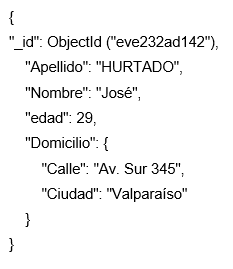
\includegraphics[ width=5cm]{./img/2.png} 
\end{center}

\textbf{¿Quiénes usan MongoDB?}\\
Existen muchas empresas que desde el 2014 usan ésta base de datos. \\
Desde Foursquare y LinkedIn o empresas de telecomunicaciones como Orange y Telefónica. \\
Empresas como Cisco, Bosch o plataformas de formación como Codecademy. \\
Otras son eBay, Expedia. Forbes, IBM, Windows Azure, McAfee  Incluso el CERN (Organización Europea para la Investigación Nuclear) utiliza MongoDB para los grandes volúmenes de datos.
\\
Finalmente podemos decir que Mongo DB es una base de datos ágil que permite a los esquemas cambiar rápidamente cuando las aplicaciones evolucionan, proporcionando siempre la funcionalidad que los desarrolladores esperan de las bases de datos tradicionales, tales como índices secundarios, un lenguaje completo de búsquedas y consistencia estricta.
\\

\textbf{Cassandra}\\
\begin{center}
	
\includegraphics[width=5cm]{./img/3.png} 
\end{center}
Cassandra es una base de datos de código abierto y que en el 2008 fue liberada por Facebook, pasando a ser de código abierto. Facebook agrego elementos a Cassandra para que las configuraciones de esta base datos fuera eficiente y económica.
Debido a la verticalidad de soluciones de datos relacionales y a la necesidad de ajustar el costo de la implementación, se diseñó Cassandra para que las configuraciones de explotación fuesen altamente escalables, horizontales y de costo bajo. 
\\
Cassandra es una base de datos escrita en Java, de tipo Column Family, diseñada por Avinash Lakshman (uno de los autores de Dynamo, de Amazon) y Prashant Malik (Ingeniero de Facebook). 
\\
Altamente escalable, eventualmente consistente, distribuida y almacenamiento estructurado llamado key-value. 
\\
Agrupa las tecnologías de sistemas distribuidos de Dynamo y el modelo de datos BigTable de Google. 
Existen varias herramientas para la visualización y administración de los datos, la más destacada es OpsCenter que ofrece gestión y administración para los cluster, esta contiene una edición comunitaria y una empresarial que incluye características adicionales: alertas, balanceo automático de cargas, respaldos en vivo, entre otras. Otras versiones: Cassandra Cluster Admin, Cassandra Explorer y Helenos.
\\
Casandra posee su Lenguaje de consulta: CQL (Cassandra Query Language), entre algunos de sus usuarios se cuentan:   Despegar, Facebook, Twitter, EBay.
Para su instalación requiere de los archivos llamados JDK que permiten compilar archivos en ambiente Java para su correcta manipulación.
En mayo del 2016, se liberó la versión 3.0 de Cassandra.
Podemos agregar finalmente que Cassandra soporta varios entornos como Python, Java, C++, C, PHP entre otros.
\\

\textbf{Lenguaje CQL}\\
Cassandra Query Language (CQL) es el lenguaje de acceso a datos en Cassandra, es un derivado reducido de SQL. \\
En Cassandra los datos están desnormalizados de manera que el concepto de joins o subqueries no existe.\\

Podemos interactuar con Cassandra mediante CQL a través de la Shell de CQL (cqlshell) También podemos usar herramientas gráficas como DevCenter o a través de los drivers soportados para múltiples lenguajes de programación.
\\

\textbf{Comandos en Cassandra:}\\


\begin{itemize}
    \item help ,connect ,create/drop keyspace ,use, 
    \item Otros: create/drop column family, set, get, list, update, truncate, show.
\end{itemize}


\textbf{Tabla comparativa entre CASSANDRA vs MongoDB}\\

\begin{center}
	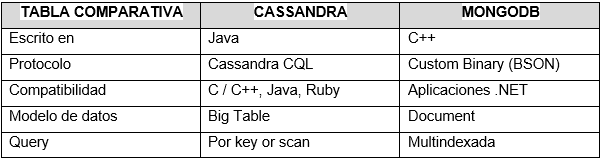
\includegraphics[width=7cm]{./img/4.png} 
\end{center}

\section{Conclusiones}
El objetivo de esta articulo es ampliar los conocimientos sobre las Bases de Datos NoSQL y comparar ciertas características respecto a las Bases de Datos Relacionales a las que se está más familiarizado, en definitiva de esta manera se llega a la conclusión que las Bases de Datos NoSQL no son un reemplazo ni superiores o inferiores a las BD Tradicionales SQL, sino que son una alternativa que ofrece otras posibilidades o beneficios para explotarlos en determinados proyectos que requieren una alta escalabilidad y que los recursos son escasos y la integridad de los datos no es lo más importante, como sí ocurre en cambio en aplicaciones especializadas como por ejemplo en transacciones bancarias que son indispensables el manejarlas con BD Relacionales.\\

\section{Recomendaciones}
No todos los sistemas de base de datos NoSQL funcionan mejor que las bases de datos relacionales. MongoDB y Cassandra tienen un rendimiento similar, y en muchos casos mejor, que en las bases de datos relacionales en operaciones de escritura y eliminación.\\

\section{Biblografia}

\begin{itemize}
    \item Pérez Fernández, Vicente y coautores. Bases de datos. Ciudad de La habana, Editorial Pueblo y Educación, 2001. \\
    https://www.ecured.cu/Base\_de\_datos\_re\\lacional 
    \item Óscar Pérez Mora, Bases de Datos.Mexico (2005) \\http://www.uoc.edu/masters/oficiales/i\\mg/913.pdf 
    \item Shashank Tiwari, John Wiley .Professional NoSQL, \& Sons, 2011. \\
    http://www.wrox.com/WileyCDA/WroxT\\itle/Professional-NoSQL.productCd-047094224X.html 
    \item Claudia Pinilla, Mauricio Bello y Cristian Peña. Bases de datos orientadas a grafos, 2017 \\
    http://revistas.udistrital.edu.co/ojs/index.\\php/tia/article/viewFile/8769/pdf
    \item Germán Romeo, “Bases de datos NoSQL”, Noviembre 2013 \\ https://www.seas.es/blog/informatica/ba\\ses-de-datos-nosql/ 
    \item Gustavo Rodriguéz, “Motores de Bases de datos”, Octubre \\ 2015 https://prezi.com/ry9ckaivktcx/mo\\tores-de-base-de-datos/ 
    \item Diego López de Ipiña, “Bases de Datos No Relacionales (NoSQL)”, Noviembre de 2012\\
     https://es.slideshare.net/dipina/bases-de-datos-no-relacionales-nosql
     \item Marin Dimitrov .”NoSQL databases”, Marzo 2010 \\ http://www.slideshare.net/marin\_dimitr\\ov/n\\osql-databases-3584443
\end{itemize}

%%%%%%%%%%%%%%%%%%%%%%%%%%%%%%%%%%%%%%%%%%%%%%%%%%%%%%%%%
\end{document}